\section{\esp Protocolo da Revisão Sistemática de Literatura }\label{protocolo}

%Definição, diferença
Segundo \citeonline{Kitchenham:2007}, uma \ac{RSL} é um método de seleção de artigos, no qual a busca por materiais bibliográficos é formalizada sistematicamente a partir da elaboração e utilização de um protocolo de busca. Uma \ac{RSL} tem como objetivos: resumir evidências empíricas, identificar lacunas existentes nas pesquisas realizadas até o momento e fornecer subsídios para realizar novas pesquisas.
Enquanto uma Revisão Literatura, também chamada de Revisão Ad-hoc, não utiliza o protocolo para a formalização da pesquisa realizada, dessa forma tornando mais difícil sua replicabilidade.

%etapas
Uma \ac{RSL} é  composta por três fases: planejamento da revisão, condução da revisão e análise dos materiais obtidos.
Na fase de planejamento define-se a pergunta de pesquisa, seleciona-se as palavras chave e determina-se os critérios de inclusão e de exclusão de materiais bibliográficos; na condução da revisão é realizado uma busca a partir da combinação das palavras chave e na última fase  é realizado um estudo dos materiais que foram obtidos. A seguir será apresentada a descrição das etapas da elaboração e a execução do protocolo de \ac{RSL} utilizado neste artigo para encontrar e selecionar os materiais que posteriormente foram estudados neste artigo.

%Protocolo da revisão
\subsection{Planejamento da Revisão}

A revisão sistemática de literatura proposta neste trabalho tem como objetivo investigar quais métricas e metodologias aplicadas ao \ac{PERE} entre 1998 e o mês de Outubro de 2016, abrangendo um período de 18 anos, de forma a responder a seguinte questão de pesquisa:

\begin{itemize}
\item \emph{Quais métricas e metodologias empregadas ao \acl{PERE} foram publicadas desde 1998 até o mês de Outubro de 2016?}
\end{itemize}

Para responder à pergunta foram consultados artigos de pesquisadores que aplicaram métricas e metodologias ao \ac{PERE}, tendo como um dos resultados esperados a relação das métricas e metodologias utilizadas no período de tempo definido na questão anterior. 

A consulta por artigos relacionados foi realizada com a utilização das seguintes palavras chave:

\begin{itemize}
\item \textit{``home health care''}
\item \textit{``home care''}
\item \textit{``nurse''}
\item \textit{``routing''}
\item \textit{``scheduling''}
\end{itemize}

Organizadas na seguinte expressão de busca:

\begin{itemize}
\item \textit{`` ( (``home health care'' OR ``home care'' OR ``nurse'') AND ``routing'' AND ``scheduling'' ) ''}
\end{itemize}

Após a elaboração da expressão de busca, foram definidos os critérios para inclusão e exclusão dos materiais bibliográficos.

\textbf{Critérios de inclusão:}

\begin{itemize}
\item Artigos relacionados ao Problema de Escalonamento e Roteamento de Enfermeiras; 
\item Artigos publicados em revistas ou conferências;
\item Artigos completos.
\end{itemize}

\textbf{Critérios de exclusão:}

\begin{itemize}
\item Artigos que foram publicados em idiomas que diferem do inglês ou português;
\item Artigos inacessíveis ou indisponíveis;
\item Artigos duplicados;
\item Artigos publicados antes de 1998.
\end{itemize}

\subsection{\esp Condução das buscas}

Após a definição dos critérios de inclusão e de exclusão dos materiais bibliográficos, foram escolhidas as seguintes bases de pesquisa, a partir da sua popularidade, para realizar as buscas:

\begin{itemize}
\item \textit{Science Direct};
\item \textit{Springer};
\item \textit{Scopus};
\item \textit{IEEE Xplore};
\item \textit{ACM Digital Library}.
\end{itemize}

Após a realização das buscas, foram retornados 158 resultados, organizados na Figura~\ref{bases}. 

\begin{figure}[ht]
\begin{center}
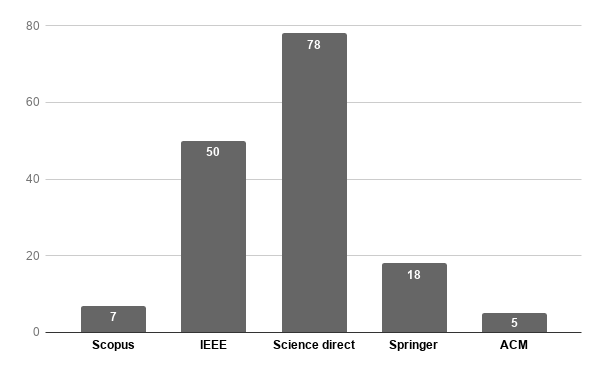
\includegraphics[width=0.4\textwidth]{base_de_dados_de_origem.png}
\caption{Contagem por bases de pesquisa \label{bases}}
\end{center}
\end{figure}


A partir da aplicação dos critérios de inclusão e de exclusão nos artigos consultados foram aceitos 19 artigos, por atenderem a todos os critérios de inclusão e 139 artigos rejeitados por atenderem a pelo menos um critério de exclusão ou por não se encaixarem em algum critério de inclusão. É interessante observar que os artigos coletados foram publicados entre os anos de 1998 e 2016, sendo que houve um aumento considerável de publicações entre os anos de 2012 e 2016, de acordo com a Figura~\ref{ano}.
 
Após a aplicação dos critérios de inclusão e exclusão nos materiais bibliográficos, foi observado que 86,7\%,  dos artigos foram rejeitados. Acredita-se que o motivo para este alto índice de rejeição seja por conta da relação do assunto estudado com publicações existentes em diversas áreas de saúde, fazendo com que as bases de pesquisa apontassem para artigos que posteriormente não se encaixariam em algum critério de inclusão. 

\begin{figure}[ht]
\begin{center}
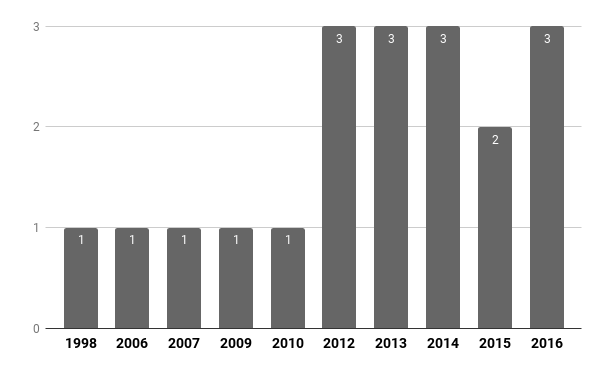
\includegraphics[width=0.4\textwidth]{contagem_por_ano.png}
\caption{Contagem de artigos por ano de publicação \label{ano}}
\end{center}
\end{figure}

